%----------------------------------------------------------------------------------------
%	PACKAGES AND THEMES
%----------------------------------------------------------------------------------------

\documentclass{beamer}

\mode<presentation> {

% The Beamer class comes with a number of default slide themes
% which change the colors and layouts of slides. Below this is a list
% of all the themes, uncomment each in turn to see what they look like.

%\usetheme{default}
%\usetheme{AnnArbor}
%\usetheme{Antibes}
%\usetheme{Bergen}
%\usetheme{Berkeley}
%\usetheme{Berlin}
%\usetheme{Boadilla}
\usetheme{CambridgeUS}
%\usetheme{Copenhagen}
%\usetheme{Darmstadt}
%\usetheme{Dresden}
%\usetheme{Frankfurt}
%\usetheme{Goettingen}
%\usetheme{Hannover}
%\usetheme{Ilmenau}
%\usetheme{JuanLesPins}
%\usetheme{Luebeck}
%\usetheme{Madrid}
%\usetheme{Malmoe}
%\usetheme{Marburg}
%\usetheme{Montpellier}
%\usetheme{PaloAlto}
%\usetheme{Pittsburgh}
%\usetheme{Rochester}
%\usetheme{Singapore}
%\usetheme{Szeged}
%\usetheme{Warsaw}

% As well as themes, the Beamer class has a number of color themes
% for any slide theme. Uncomment each of these in turn to see how it
% changes the colors of your current slide theme.

%\usecolortheme{albatross}
%\usecolortheme{beaver}
%\usecolortheme{beetle}
%\usecolortheme{crane}
%\usecolortheme{dolphin}
%\usecolortheme{dove}
%\usecolortheme{fly}
%\usecolortheme{lily}
%\usecolortheme{orchid}
%\usecolortheme{rose}
%\usecolortheme{seagull}
%\usecolortheme{seahorse}
%\usecolortheme{whale}
%\usecolortheme{wolverine}

%\setbeamertemplate{footline} % To remove the footer line in all slides uncomment this line
%\setbeamertemplate{footline}[page number] % To replace the footer line in all slides with a simple slide count uncomment this line

%\setbeamertemplate{navigation symbols}{} % To remove the navigation symbols from the bottom of all slides uncomment this line
}

\usepackage{graphicx} % Allows including images
\usepackage{booktabs} % Allows the use of \toprule, \midrule and \bottomrule in tables
\usepackage{extarrows}%arrow
\usepackage{CJKutf8} %支持中文
\usepackage{enumerate}
\usepackage{amssymb}
\usepackage{algorithm}
\usepackage{algorithmic} 
\usepackage{amsmath}

\begin{document}

%------------------------------------------------------------------------------
%    中文支持
%------------------------------------------------------------------------------
\begin{CJK*}{UTF8}{} %中文支持
\CJKfamily{gbsn} %中文支持

%----------------------------------------------------------------------------------------
%	TITLE PAGE
%----------------------------------------------------------------------------------------

\title[哈尔滨工程大学~国家保密学院]{基于变异的SQL注入漏洞测试技术的\\研究与仿真实现}
%\title[Short title]{Full Title of the Talk Bayes} % The short title appears at the bottom of every slide, the full title is only on the title page

\author{汪 \ 诚 \ 弘}
%\author{John Smith} % Your name
\institute[2011212116] % Your institution as it will appear on the bottom of every slide, may be shorthand to save space
{
%信息安全(保密技术)\\
%国 ~~ 家 ~~ 保 ~~ 密 ~~ 学 ~~ 院 \\ % Your institution for the title page
 \begin{flushleft}
~~~~~~~~~~~~~~~~~~~~~~~~~~~~~~~~~~~~~~~~~~~~ 院 ~~~~~ 系:国家保密学院 \\
\medskip
~~~~~~~~~~~~~~~~~~~~~~~~~~~~~~~~~~~~~~~~~~~~ 专 ~~~~~ 业:信息安全(保密技术)\\
\medskip
~~~~~~~~~~~~~~~~~~~~~~~~~~~~~~~~~~~~~~~~~~~~ 学 ~~~~~ 号:2011212116 \\
\medskip
~~~~~~~~~~~~~~~~~~~~~~~~~~~~~~~~~~~~~~~~~~~~ 指导老师:赵 ~~ 靖 ~~教授 \\
\end{flushleft}
%\leftline{院系:国家保密学院} \\
%\leftline{专业:信息安全(保密技术)} \\
%\leftline{学号:2011111223} \\
%\leftline{指导老师:赵靖} \\
%\medskip
%\medskip
%\textit{zhangdonghong@hrbeu.edu.cn} % Your email address
}
\date{\today} % Date, can be changed to a custom date

\begin{frame}
\titlepage % Print the title page as the first slide
\end{frame}

%----------------------------------------------------------------------------------------
%	概述
%----------------------------------------------------------------------------------------

\begin{frame}
\frametitle{论文结构}
\tableofcontents 
\end{frame}

%------------------------------------------------
%	研究背景
%------------------------------------------------

\section{概述}
\begin{frame}
\frametitle{What is SQLi?}
\begin{figure}  
 \centering  
 \includegraphics[width=90mm]{sqli.png}\\  
 %\caption{Experiment Architecture.}  
% \label{fig:env}  
\end{figure}
\end{frame}

\begin{frame}
\frametitle{What is SQLi?}
\begin{block}{交通部违章车辆号牌登记程序代码}
\emph{mysql = \\'INSERT INTO TABLICE.ILLNO (NO, Min, Max) VALUES ('\\
+var1+','+var2+','+var3+')'\bigskip\\
{\bf e.g.} var1 = ZU666, var=120, var=170,\\
mysql = \\'INSERT INTO TABLICE.ILLNO (NO, Min, Max) VALUES (ZU666,120,170)'}
\end{block}
\begin{block}{SQLi Attack}
\emph{mysql = \\'INSERT INTO TABLICE.ILLNO (NO, Min, Max) VALUES (ZU666,0,0);\\DROP DATABASE TABLICE'\\}
--,120,170)'
\end{block}

\end{frame}

%------------------------------------------------------------------------------------------


\begin{frame}
\frametitle{研究背景}
\begin{block}{SQL Injection}
SQLi(SQL injection)漏洞是WEB2.0和HTML5时代最危险地WEB应用程序漏洞,该漏洞主要由于数据库驱动的WEB应用程序对用户输入检查不严格,导致用户可以注入SQL命令从而任意执行恶意代码。
\end{block}
\begin{itemize}
\item 高威胁性, 5年OWASP威胁榜榜首
\item 普遍性和频发性, NGS公司安全白皮书显示,世界几乎没3分钟就会发生一次SQLi攻击
\end{itemize}
\end{frame}

%--------------------------------------------------------------

\begin{frame}
\frametitle{国内外研究现状}
\begin{block}{国际领域研究现状}
~~~~目前国际领域的研究主要形成了4种主流的SQLi防御理论:动态监测(Runtime Monitor),静态分析(Static Analysis),混合防御(Hybrid Approach),漏洞测试(Vulnerability Testing)。目前国际领域公认的最可靠最高效的防御方式是{\bf 漏洞测试}的方法。\\
\begin{table}
\begin{tabular}{l l}
\toprule
\textbf{Method} & \textbf{Evaluation}\\
\midrule
RM & 监测开销巨大,程序可用性降低(Zhang et.al.) \\
SA & 误报率高,信息收集不完全(William el.al.) \\
HA & 实现困难,过程繁琐 \\
VT & 测试效率相对较低,测试执行时间长\\
\bottomrule
\end{tabular}
\caption{SQLi防御机制比较}
\end{table}
\end{block}

\end{frame}



\begin{frame}
\frametitle{研究内容}
\begin{block}{集中解决的问题}
\medskip
(1)测试用例状态空间爆炸,测试漏洞的测试用例往往有上万条\\
\medskip
\medskip
(2)有效测试用例分布稀疏,即测试用例的有效度低\\
\medskip
\medskip
(3)执行测试的开销较高,执行每一条测试用例必须需要人工参与\\
\medskip
\end{block}
\begin{block}{提出的解决方案}
$$Do ~Fewer~~~ Search~ Faster$$
$$MU4SQLi$$
\end{block}
\end{frame}
\begin{frame}
\frametitle{MU4SQLi}
\begin{figure}  
 \centering  
 \includegraphics[width=120mm]{liucheng.png}\\  
 %\caption{Experiment Architecture.}  
% \label{fig:env}  
\end{figure}
\end{frame}

%--------------------------------------------------------------
%	主要内容
%--------------------------------------------------------------

\section{基于变异的测试用例生成技术}
\begin{frame}
\frametitle{}
$$Mutation ~Based~$$ $$ Test ~Case ~Generation$$

\end{frame}
%---------------------------------------------------------------
\begin{frame}
\frametitle{变异测试用例生成技术}
~~~~假设程序$P$是待测程序,测试用例空间为$T=\{t_{1},t_{2},...,t_{n}\}$,我们将其设为初始状态空间。定义变异操作符空间$MO=\{mo_{1},mo_{2},..,mo_{k}\}$表示所有的变异操作符。我们将$T$中的每一个测试用例与$MO$中的每一个变异操作符结合,生成不重复的测试用例空间$T'$的过程叫做变异测试用例生成过程。\bigskip\\
\end{frame}

%---------------------------------------------------------------


\begin{frame}
\frametitle{MU4SQLi中的变异操作符}
\begin{figure}  
 \centering  
 \includegraphics[width=100mm]{1.jpg}\\  
 %\caption{Experiment Architecture.}  
% \label{fig:env}  
\end{figure}

\end{frame}

\begin{frame}
\frametitle{MU4SQLi变异测试用例生成算法}
\begin{figure}  
 \centering  
 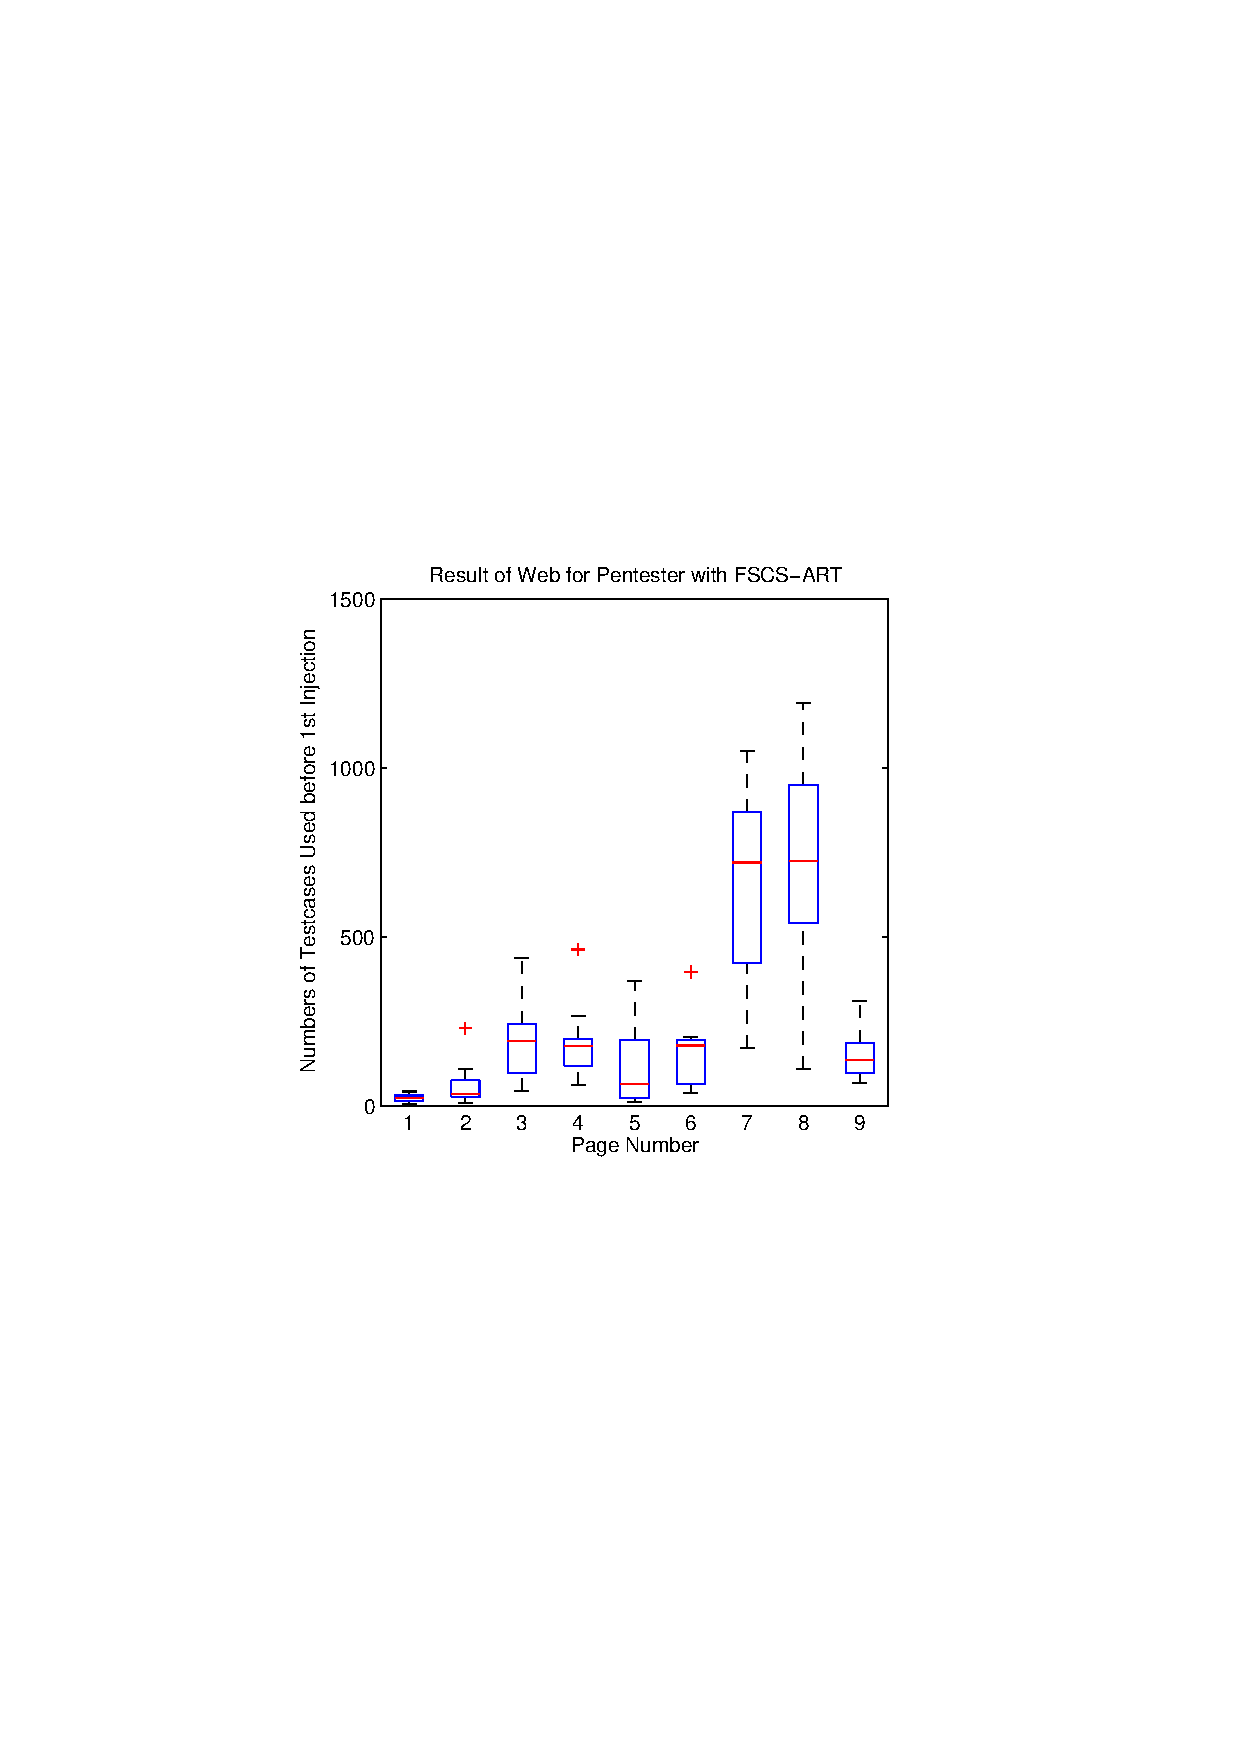
\includegraphics[width=85mm]{2.png}\\  
 %\caption{Experiment Architecture.}  
% \label{fig:env}  
\end{figure}

\end{frame}

\begin{frame}
\frametitle{	MU4SQLi测试用例生成特点}
\begin{itemize}
\item 测试用例有效度高,能够消除认为设计的不足
\item 测试用例状态空间巨大,变异程度越高
\end{itemize}

\end{frame}

\section{自适应随机选择方法}
\begin{frame}
\frametitle{}
$$Adaptive~ Random $$ $$Method~ Based ~Selection$$

\end{frame}

\begin{frame}
\frametitle{SQLi有效测试用例分布}
~~~~能够触发SQLi漏洞的测试用例往往都具有很高的字串相似度。即从字串结构的角度去观察,有效测试用例呈现出聚类的特性。
\begin{table}
\begin{tabular}{l l}
\toprule
\textbf{No.} & \textbf{Successful Test Cases for CVE2014-3704} \\
\midrule
1 & ; or 1 = 1 waitfor delay '0: 0: TIME -- \\
2 & ); or 1 = 1 waitfor delay '0: 0: TIME -- \\
3 & '; or 1 = 1 waitfor delay '0: 0: TIME -- \\
4 & ''; or 1 = 1 waitfor delay '0: 0: TIME -- \\
5 & '); or 1 = 1 waitfor delay '0: 0: TIME -- \\
... & ... \\
\bottomrule
\end{tabular}
\caption{Successful Test Cases for CVE2014-3704}
\end{table}
\end{frame}


%\begin{frame}
%\frametitle{Preliminary Experiment}
%In order to describe the previous observation consequences of the successful SQLi test cases distribution,we apply the TF-IDF algorithm to compute the test cases distance.In other words, we use the values of TF-IDF  to quantify the similarity of between test cases.\\~\\
%TF-IDF is the abbreviation of term frequency–inverse document frequency.Then tf–idf is calculated as:\\
%$$\mathrm{tfidf_{i,j}} = \mathrm{tf_{i,j}} \times \mathrm{idf_i}$$
%$$\mathrm{tf_{i,j}}= \frac{n_{i,j}}{\sum_k n_{i,j}}$$
%$$ \mathrm{idf_i}=  \log \frac{|D|}{|\{j : t_i \in d_j\}|}$$
%\end{frame}


\begin{frame}
\frametitle{解决方案}
~~~~我们提出了一种基于自适应随机 {\bf Adaptive Random} 思想的SQLi漏洞待测用例选择技术,该技术能够快速收敛到有效测试用例。下面给出具体的实施步骤:\bigskip\\
\begin{enumerate}[Step 1]
\item 利用TF-IDF技术提取测试用例的特征向量(eq 3.1).
\item 利用PCA方法进行测试用例向量降维(eq 3.2-3.11).
\item 利用Cosine距离定义测试用例距离测度(eq 3.12 3.13).
\item 利用FSCS(Fixed Size Candidate Set)算法进行待测用例筛选.
\end{enumerate}
\end{frame}
\begin{frame}
\frametitle{MU4SQLi的FSCS 算法 -- $S_{distance}$ 选择算法}
 $E = \{e_{1}, e_{2}, e_{3}, ..., e_{f}\}$ 已执行测试用例集\\ $C= \{c_{1}, c_{2}, c_{3}, ..., c_{\kappa}\}$ 候选集合\bigskip\\
 而待测用例$c_{h}$的选择需满足以下的条件:
$For~ all ~ j~ \in~ \{1, 2, 3, ..., \kappa\} $, $$\min_{i=1}^{f} dis(c_{h}, e_{i}) \geq \min_{i=1}^{f} dis(c_{j}, e_{i}) $$
\end{frame}






%-----------------------------------------------------------------

\section{仿真测试}
\begin{frame}
$$Simulation~Evaluation$$
\end{frame}
%----------------------------------------------------------------
%	Thank you
%----------------------------------------------------------------

\begin{frame}
~~~~为了验证我们设计的MU4SQLi测试框架的测试用例有效度和测试效率,我们需要进行实际的比对测试。将MU4SQLi与传统的测试方法进行比对,并且比较传统测试方法在测试有效度和测试效率上运行性能。由于实际环境下的测试对于资源的消耗非常巨大。并且,对于安全测试来说Test Oracle问题(Test Oracle Problem)仍是一个困扰安全测试的关键性问题。因此我们选择利用仿真测试评估MU4SQL i
\end{frame}

\begin{frame}
\frametitle{仿真平台搭建}
我们的仿真平台如下图所示:\\
\begin{figure}  
 \centering
 \includegraphics[width=85mm]{vm.png}\\  
 %\caption{Experiment Architecture.}  
% \label{fig:env}  
\end{figure}
\end{frame}
\begin{frame}
\frametitle{仿真平台搭建}
下表给出了仿真平台中各仿真模块和仿真SUT的具体配置:\\
\begin{figure}  
 \centering  
 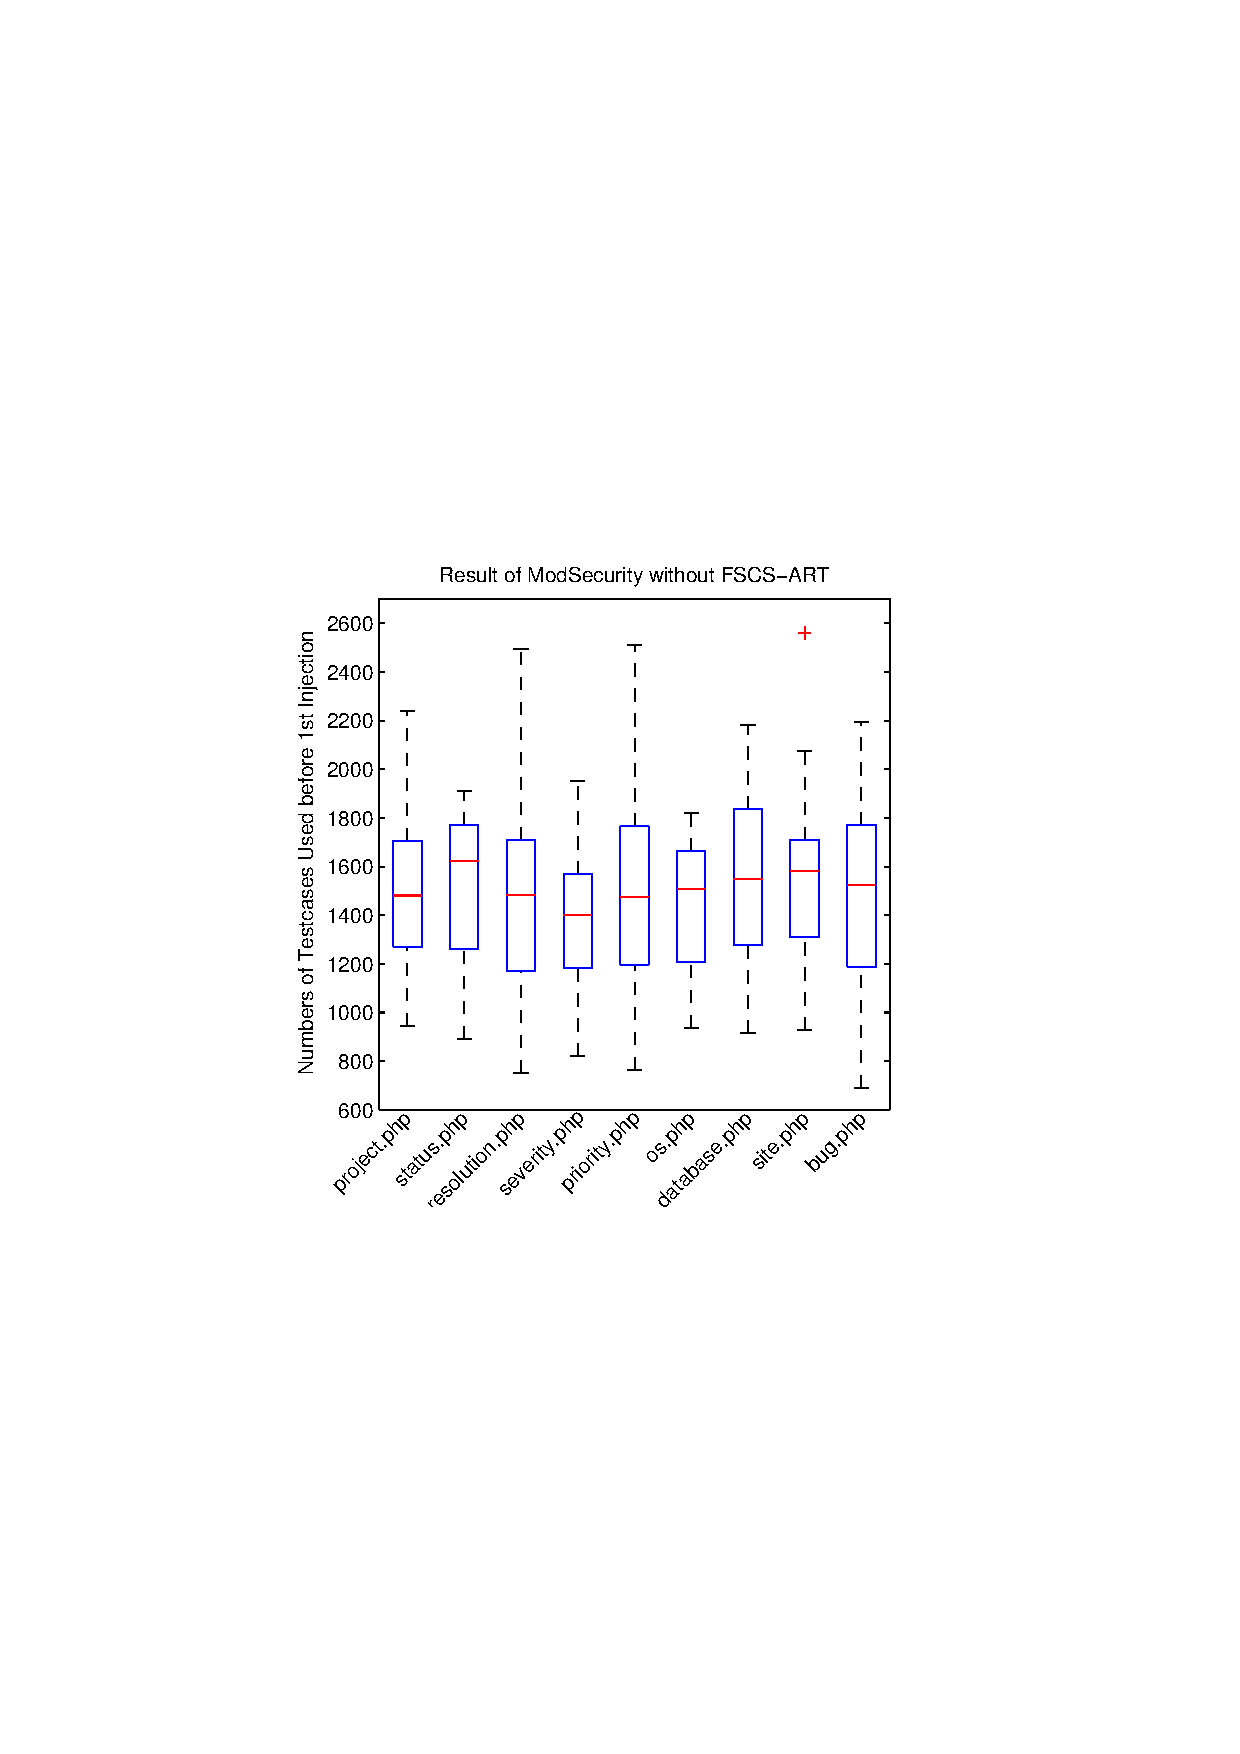
\includegraphics[width=100mm]{5.png}\\  
 %\caption{Experiment Architecture.}  
% \label{fig:env}  
\end{figure}
\end{frame}
%----------------------------------------------------------------------------------------
%	END
%------------------------------------------------------------------------------------------
\begin{frame}
\frametitle{测试用例有效性仿真结果}
测试用例有效度仿真测试结果:\\
\begin{figure}  
 \centering  
 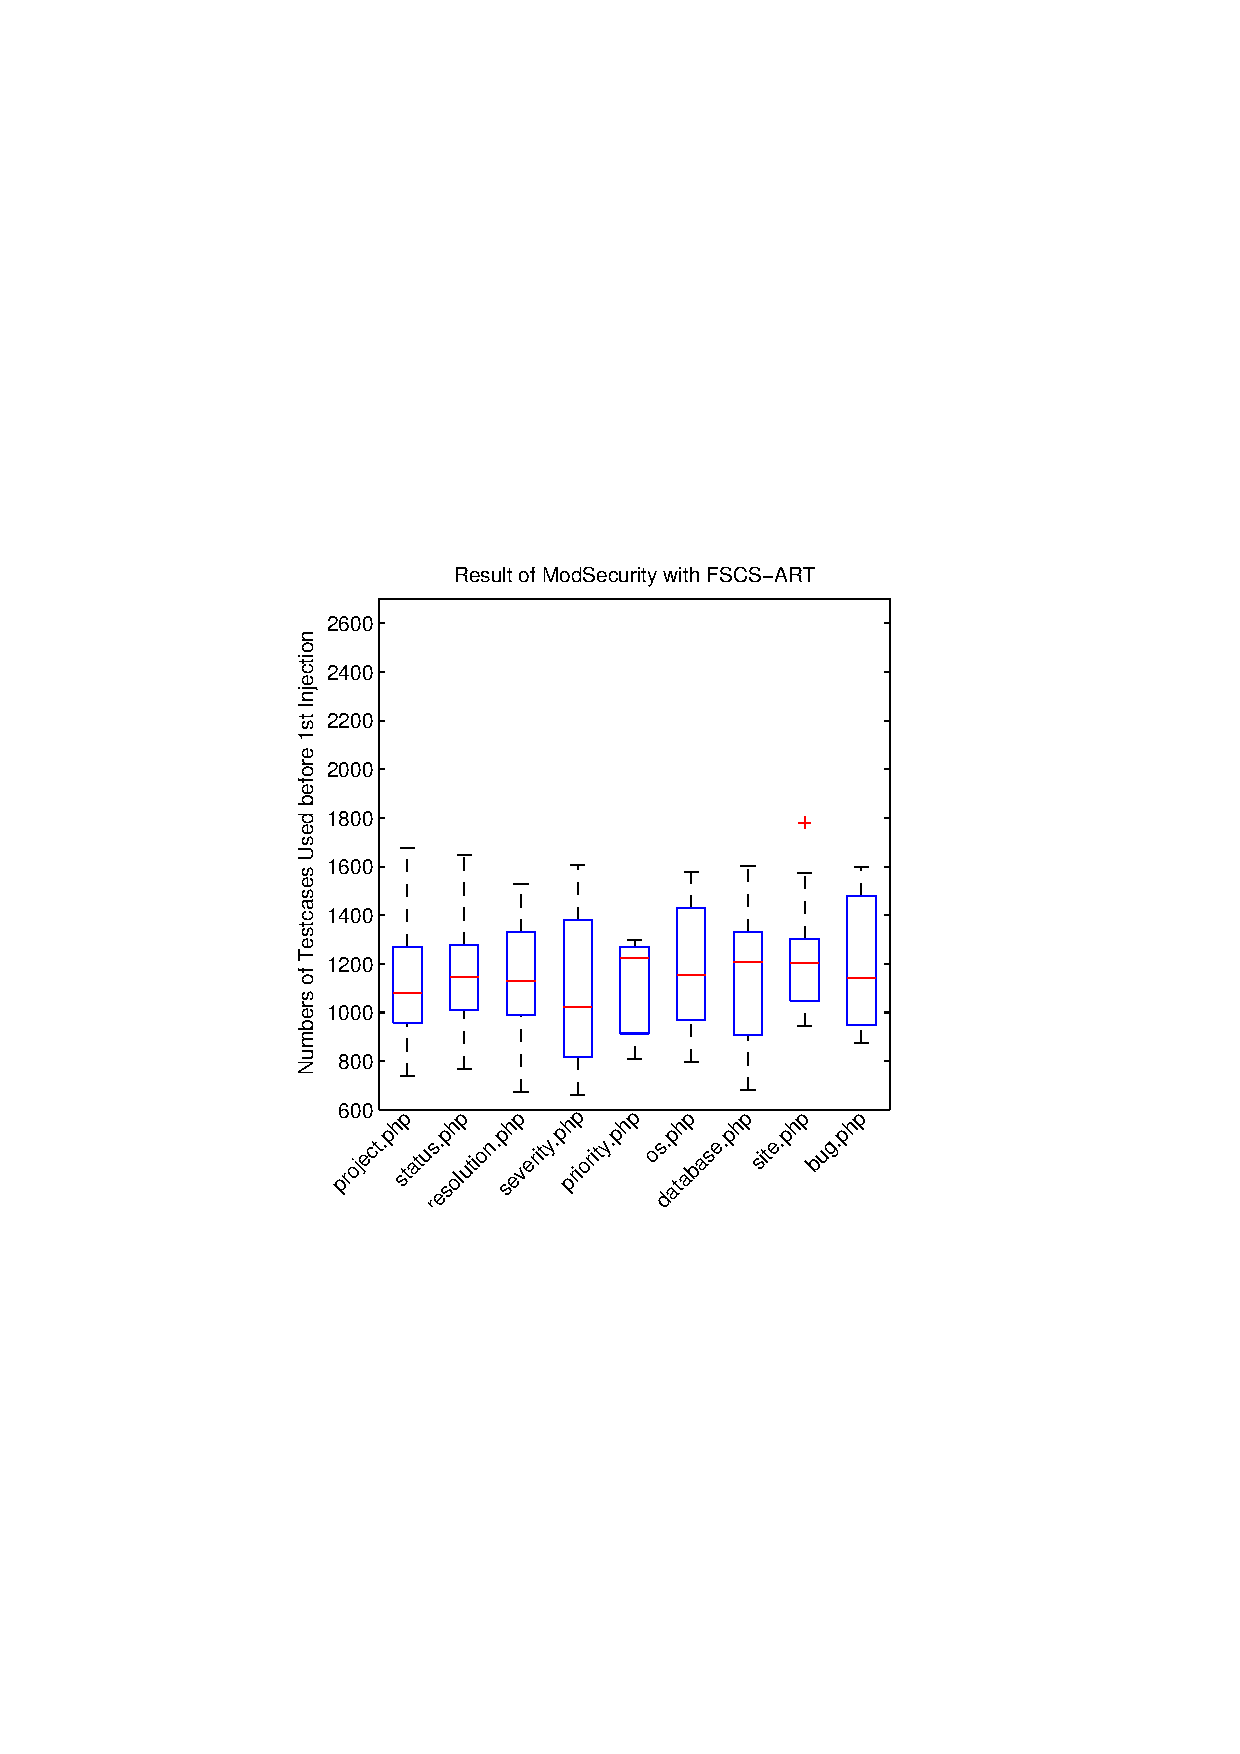
\includegraphics[width=100mm]{6.png}\\  
 %\caption{Experiment Architecture.}  
% \label{fig:env}  
\end{figure}
上图中左边图为Web for Pentester测试平台右边为SPB测试平台。图中绿色的线代表传统测试,蓝色的线代表基于变异的测试用例生成技术。很明显,变异生成的测试用例有效度远高于传统测试模式。
\end{frame}

\begin{frame}
\frametitle{测试执行效率仿真对比测试W4P}
测试执行效率仿真对比测试W4P:\\
\begin{figure}  
 \centering  
 \includegraphics[width=100mm]{7.png}\\  
 %\caption{Experiment Architecture.}  
% \label{fig:env}  
\end{figure}
\end{frame}
\begin{frame}
\frametitle{测试执行效率仿真对比测试SPB}
测试执行效率仿真对比测试SPB:\\
\begin{figure}  
 \centering  
 \includegraphics[width=100mm]{8.png}\\  
 %\caption{Experiment Architecture.}  
% \label{fig:env}  
\end{figure}
\end{frame}

\begin{frame}
\frametitle{测试执行效率仿真对比测试AVG-Fmeasure}
测试执行效率仿真对比测试AVG-Fmeasure:\\
\begin{figure}  
 \centering  
 \includegraphics[width=100mm]{9.png}\\  
 %\caption{Experiment Architecture.}  
% \label{fig:env}  
\end{figure}
在执行效率方面,自适应随机的方法也非常有效,从图中可以看出,我们的方法较传统测试方法提升平均20\%-30\%
\end{frame}
\begin{frame}
$$Thank ~You$$
\end{frame}
\begin{frame}
\titlepage % Print the title page as the first slide
\end{frame}

%----------------------------------------------------------------------------------------

\end{CJK*}
\end{document} 